% Drawing 154/09-8 -- folder 154, batch 09, archive page 172 (PDF page 173).
% Transcription: sur une feuille de listing imprimée, deux dessins en couleur sans texte : à gauche, trois disques accolés en chaîne, bordés de vert clair et de vert foncé, traversés de pseudo-droites rouges qui se croisent de l'un à l'autre, petits triangles coloriés en jaune ; à droite, une droite vert clair coupée de quatre droites rouges (deux croisées, deux simples), qui monte en passant par le deuxième croisement, doublée de tirets vert foncé et gris et de tirets bleus, avec une flèche vers la gauche et une vers la droite. Au crayon, un cercle en tirets et deux petits triangles
% Kind: three disks glued in a chain with arrangements and yellow triangles; crossings on a line with parallels. Method 2 (schematic redraw from the facsimile). Status: partial.
% Notes: On a printed listing (CRAY2 job banner, 17 Aug 82; not reproduced), two colour drawings without text, read from the page view: left, three disks glued in a chain, bordered in light and dark green, crossed by red pseudolines that cross from one to the next, small triangles coloured yellow (drawn as wedges); right, red lines crossing on a light green line, accompanied by dark green, light green and dashed parallels which change sides at a crossing, and two red verticals; a small arrow to the left. Strands schematic; the pencil sketch above is left out.
% Coordinates: 1 unit = 1 mm = 1/100 of the crop width (bbox in page fractions: [0.216, 0.364, 0.864, 0.509]).
% Redrawn by Claude (claude-opus-5-5), issue #73, 2026-11-07; not checked by a human; not compiled (no TeX in the session).
% Rights: reproduces part of the work -- behind RENDER_TRANSCRIPTS, never published by itself.
\documentclass[tikz,border=3pt]{standalone}
\usepackage{amsmath,amssymb}
\usetikzlibrary{patterns,arrows.meta}
\tikzset{Or/.style={orange!90!black}, Ye/.style={yellow!80!orange}, Lg/.style={green!60!black!70}, Dg/.style={green!45!black}, Br/.style={brown!80!black}, Rd/.style={red!85!black}, Bl/.style={blue!70!black}, Gy/.style={black!40}, pencil/.style={black!45}, struck/.style={black!35}, mark/.style={circle,draw,inner sep=1.3pt}, pt/.style={circle,fill,inner sep=0.9pt}, opt/.style={circle,draw,fill=white,inner sep=1.1pt}}
\begin{document}
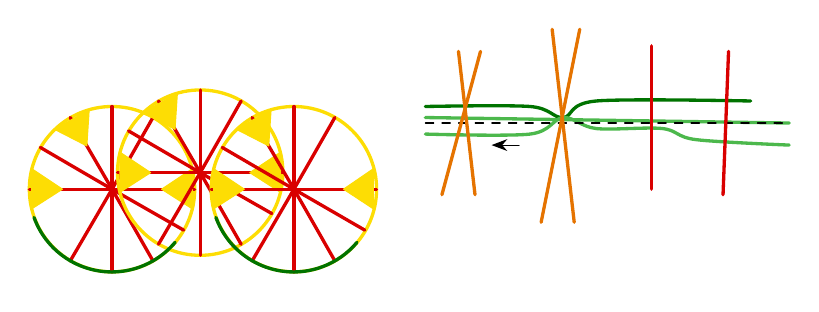
\begin{tikzpicture}[x=1mm,y=1mm,line cap=round,line join=round,font=\scriptsize]
\draw[Ye,very thick] (11.9,-21) circle[radius=10.5];
\draw[Rd,very thick] plot[smooth, tension=0.55] coordinates {(11.9,-10.5) (11.9,-21) (11.9,-31.5)};
\draw[Rd,very thick] plot[smooth, tension=0.55] coordinates {(17.1,-11.9) (11.9,-21) (6.6,-30.1)};
\draw[Rd,very thick] plot[smooth, tension=0.55] coordinates {(6.6,-11.9) (11.9,-21) (17.1,-30.1)};
\draw[Rd,very thick] plot[smooth, tension=0.55] coordinates {(1.4,-21) (11.9,-21) (22.4,-21)};
\draw[Rd,very thick] plot[smooth, tension=0.55] coordinates {(2.8,-15.7) (11.9,-21) (21,-26.2)};
\draw[Ye] (1.7,-18.4) -- (1.7,-23.5) -- (5.6,-21) -- cycle;
\fill[pattern=north east lines,Ye] (1.7,-18.4) -- (1.7,-23.5) -- (5.6,-21) -- cycle;
\draw[Ye] (22.1,-23.5) -- (22.1,-18.4) -- (18.2,-21) -- cycle;
\fill[pattern=north east lines,Ye] (22.1,-23.5) -- (22.1,-18.4) -- (18.2,-21) -- cycle;
\draw[Ye] (9,-10.9) -- (4.6,-13.4) -- (8.7,-15.5) -- cycle;
\fill[pattern=north east lines,Ye] (9,-10.9) -- (4.6,-13.4) -- (8.7,-15.5) -- cycle;
\draw[Ye,very thick] (23.1,-18.9) circle[radius=10.5];
\draw[Rd,very thick] plot[smooth, tension=0.55] coordinates {(23.1,-8.4) (23.1,-18.9) (23.1,-29.4)};
\draw[Rd,very thick] plot[smooth, tension=0.55] coordinates {(28.3,-9.8) (23.1,-18.9) (17.8,-28)};
\draw[Rd,very thick] plot[smooth, tension=0.55] coordinates {(17.8,-9.8) (23.1,-18.9) (28.3,-28)};
\draw[Rd,very thick] plot[smooth, tension=0.55] coordinates {(12.6,-18.9) (23.1,-18.9) (33.6,-18.9)};
\draw[Rd,very thick] plot[smooth, tension=0.55] coordinates {(14,-13.6) (23.1,-18.9) (32.2,-24.1)};
\draw[Ye] (12.9,-16.3) -- (12.9,-21.4) -- (16.8,-18.9) -- cycle;
\fill[pattern=north east lines,Ye] (12.9,-16.3) -- (12.9,-21.4) -- (16.8,-18.9) -- cycle;
\draw[Ye] (33.3,-21.4) -- (33.3,-16.3) -- (29.4,-18.9) -- cycle;
\fill[pattern=north east lines,Ye] (33.3,-21.4) -- (33.3,-16.3) -- (29.4,-18.9) -- cycle;
\draw[Ye] (20.2,-8.8) -- (15.8,-11.3) -- (19.9,-13.4) -- cycle;
\fill[pattern=north east lines,Ye] (20.2,-8.8) -- (15.8,-11.3) -- (19.9,-13.4) -- cycle;
\draw[Ye,very thick] (35,-21) circle[radius=10.5];
\draw[Rd,very thick] plot[smooth, tension=0.55] coordinates {(35,-10.5) (35,-21) (35,-31.5)};
\draw[Rd,very thick] plot[smooth, tension=0.55] coordinates {(40.2,-11.9) (35,-21) (29.7,-30.1)};
\draw[Rd,very thick] plot[smooth, tension=0.55] coordinates {(29.7,-11.9) (35,-21) (40.2,-30.1)};
\draw[Rd,very thick] plot[smooth, tension=0.55] coordinates {(24.5,-21) (35,-21) (45.5,-21)};
\draw[Rd,very thick] plot[smooth, tension=0.55] coordinates {(25.9,-15.7) (35,-21) (44,-26.2)};
\draw[Ye] (24.8,-18.4) -- (24.8,-23.5) -- (28.7,-21) -- cycle;
\fill[pattern=north east lines,Ye] (24.8,-18.4) -- (24.8,-23.5) -- (28.7,-21) -- cycle;
\draw[Ye] (45.1,-23.5) -- (45.1,-18.4) -- (41.3,-21) -- cycle;
\fill[pattern=north east lines,Ye] (45.1,-23.5) -- (45.1,-18.4) -- (41.3,-21) -- cycle;
\draw[Ye] (32.1,-10.9) -- (27.7,-13.4) -- (31.8,-15.5) -- cycle;
\fill[pattern=north east lines,Ye] (32.1,-10.9) -- (27.7,-13.4) -- (31.8,-15.5) -- cycle;
\draw[Dg,very thick] (2,-24.6) arc[start angle=200, end angle=320, x radius=10.5, y radius=10.5];
\draw[Dg,very thick] (25.1,-24.6) arc[start angle=200, end angle=320, x radius=10.5, y radius=10.5];
\draw[Lg,very thick] (51.7,-11.9) -- (97.9,-12.6);
\draw[Dg,very thick] plot[smooth, tension=0.55] coordinates {(51.7,-10.5) (65,-10.5) (69.2,-11.9) (73.4,-9.8) (93,-9.8)};
\draw[Lg,very thick] plot[smooth, tension=0.55] coordinates {(51.7,-14) (65,-14) (69.2,-11.9) (73.4,-13.3) (81.8,-13.3) (86,-14.7) (97.9,-15.4)};
\draw[dashed] (51.7,-12.6) -- (97.9,-12.6);
\draw[Or,very thick] (53.8,-21.7) -- (58.7,-3.5);
\draw[Or,very thick] (55.9,-3.5) -- (58,-21.7);
\draw[Or,very thick] (66.4,-25.2) -- (71.3,-0.7);
\draw[Or,very thick] (67.8,-0.7) -- (70.6,-25.2);
\draw[Rd,very thick] (80.4,-2.8) -- (80.4,-21);
\draw[Rd,very thick] (90.2,-3.5) -- (89.5,-21.7);
\draw[-{Stealth[length=2mm]}] (63.6,-15.4) -- (60.1,-15.4);
\end{tikzpicture}
\end{document}
